\documentclass[conference]{IEEEtran}
\IEEEoverridecommandlockouts
% The preceding line is only needed to identify funding in the first footnote. If that is unneeded, please comment it out.
\usepackage{cite}
\usepackage{amsmath,amssymb,amsfonts}
\usepackage{algorithmic}
\usepackage{graphicx}
\usepackage{textcomp}
\usepackage{xcolor}
\usepackage{booktabs}
\usepackage{tabularx}
\usepackage{url}
\usepackage[utf8]{inputenc}
\usepackage[spanish,es-tabla]{babel}

\def\BibTeX{{\rm B\kern-.05em{\sc i\kern-.025em b}\kern-.08em
    T\kern-.1667em\lower.7ex\hbox{E}\kern-.125emX}}

\begin{document}

\title{Predicción de Tiempos Muertos y Clasificación Automatizada de Tickets de Mantenimiento Mediante Aprendizaje Computacional en la Industria de Manufactura\\
{\footnotesize \textsuperscript{*}Proyecto de Optimización Operativa en Planta de Moldeo por Inyección (Flex Guadalajara Norte)}}

\author{
\IEEEauthorblockN{Juan Pablo Torres Guillen}
\IEEEauthorblockA{Matrícula: A01743268 \\
\textit{Tecnológico de Monterrey} \\
Guadalajara, Jalisco, México}
\and
\IEEEauthorblockN{Angel David Lugo Lafarga}
\IEEEauthorblockA{Matrícula: A01741564 \\
\textit{Tecnológico de Monterrey} \\
Guadalajara, Jalisco, México}
\and
\IEEEauthorblockN{Jose Pablo Lopez Rodriguez}
\IEEEauthorblockA{Matrícula: A01638911 \\
\textit{Tecnológico de Monterrey} \\
Guadalajara, Jalisco, México}
}

\maketitle

\begin{abstract}
En una planta de manufactura, que las máquinas estén disponibles es clave para cumplir con la producción. En el área de moldeo por inyección de Flex Guadalajara Norte, el mantenimiento correctivo enfrenta dos problemas: los paros de máquina (\textit{downtime}) tienen duraciones muy variables y no se sabe con anticipación qué equipos van a requerir atención, y el registro de fallas no está estandarizado, por lo que casi un tercio del tiempo muerto no tiene una causa registrada. Este documento presenta la introducción, la descripción de los problemas a resolver (identificación de equipos críticos con predicción de fallas, y clasificación automática del texto de cierre de los tickets), la descripción del conjunto de datos, el preprocesamiento exhaustivo para la predicción de \textit{downtime} y el mapeo/armonización de columnas entre sistemas, y los principales resultados del análisis exploratorio de datos (EDA). El EDA muestra que el 72\% del tiempo muerto se concentra en máquinas de inyección (IMM) y robots, que el 29\% de las horas de paro ocurre durante cambios de molde (mediana de 0.66~h) y que es posible unir 4,928 tickets entre ambas fuentes para construir modelos de clasificación de texto, regresión y agrupamiento.
\end{abstract}

\begin{IEEEkeywords}
Downtime prediction, text classification, exploratory data analysis, predictive maintenance, injection molding, natural language processing.
\end{IEEEkeywords}

\section{Introducción}
En la manufactura electrónica y de moldeo por inyección se trabaja con esquemas de producción \textit{Just-in-Time} (JIT), donde cualquier paro no planeado de una máquina genera pérdidas económicas, retrasos con los clientes y baja la eficiencia global del equipo (\textit{Overall Equipment Effectiveness}, OEE). Por eso, el mantenimiento industrial ha pasado de ser solo reactivo a usar análisis de datos y aprendizaje automático para anticipar fallas~\cite{mobley2002,jardine2006}.

En la planta de Flex Guadalajara Norte, en la nave de Moldeo, operan alrededor de 80 máquinas de inyección de plástico (\textit{Injection Molding Machines}, IMM) junto con robots cartesianos, termorreguladores, secadores y otros equipos periféricos; en los registros aparecen 92 equipos en total. De acuerdo con el socio formador, actualmente solo unas 35 máquinas están en operación, mientras que el resto tiene paro programado por baja demanda. La planta registra los paros de máquina y las solicitudes de mantenimiento correctivo en dos sistemas distintos. Como parte de la captura es manual y los dos sistemas no siempre coinciden, hay inconsistencias en los datos y se pierde trazabilidad de algunas fallas.

El objetivo del proyecto es aprovechar el historial de paros y tickets de la planta, incluyendo el texto libre que escriben operadores y técnicos, para generar información útil para el equipo de mantenimiento.

\subsection{Descripción de los Problemas a Resolver}
A partir de los datos entregados y de la sesión de preguntas con el socio formador, se definieron dos problemas principales:

\subsubsection{Identificación de Equipos Críticos y Predicción de Fallas}
El socio formador indicó que su prioridad es identificar los equipos que requieren atención y, además de prevenir, predecir las fallas. Actualmente la duración de los paros varía mucho (desde microparos de pocos minutos hasta paros de más de 60 horas), y no hay una forma sistemática de anticipar qué máquinas van a acumular más tiempo muerto. Para Flex, un problema es importante cuando representa alrededor del 20\% de su tiempo muerto semanal, y la gravedad de un paro no se define con un umbral fijo de horas: depende del tipo de máquina y de falla (por ejemplo, un paro de 6--7 horas se considera grave).

Para atender este problema se plantea: (a) agrupar las máquinas según su comportamiento de fallas (frecuencia, tiempo promedio de reparación y tiempo entre fallas) para identificar las que requieren atención, y (b) predecir el número de paros y las horas de paro por máquina, así como la duración esperada de un paro. Como la duración tiene un fuerte sesgo a la derecha, se usarán transformaciones de escala y modelos robustos, con variables como el tipo de equipo, la máquina, el motivo del paro y el turno.

\subsubsection{Clasificación del Texto de Cierre (Columna Q) en la Categoría Dispositivo (Columna AB)}
En la base de tickets, el técnico describe en texto libre lo que hizo al cerrar el ticket (columna Q, \texttt{Work Description (Close Details)}) y asigna manualmente una categoría del componente involucrado (columna AB, \texttt{Dispositivo}). Esta categoría tiene 44\% de valores vacíos y 557 variantes escritas de forma distinta (por ejemplo, \textit{Installation} e \textit{installation}). Según el socio formador, las categorías vacías o en ``0'' corresponden a tickets que el técnico no cerró, y el catálogo de categorías es cerrado, por lo que no se pueden agregar categorías nuevas.

El problema consiste en construir un algoritmo que reciba el texto de la columna Q y regrese la categoría de la columna AB, usando los 5,222 tickets que tienen ambos datos. Esto permitiría completar los tickets sin categoría y sugerir la categoría al técnico al cerrar un ticket.

\section{Dataset}
Se utilizaron dos archivos de Microsoft Excel entregados por el socio formador, con registros de enero de 2025 a agosto de 2026.

\subsection{Fuentes de Datos}
\begin{enumerate}
    \item \textbf{Base de Tickets de Mantenimiento (\texttt{Clasificacion de Tickets 2021.xlsm}):} Contiene las órdenes de mantenimiento correctivo. Su hoja principal, \texttt{Data}, tiene 11,150 filas (11,112 tickets únicos) y 42 columnas. Las variables principales son el número de ticket (\texttt{Number}, p.~ej., \textit{REQ-1761298}), la máquina (\texttt{Equipment Name}), las fechas de apertura y cierre (\texttt{Opened}, \texttt{Updated}), el tiempo de reparación capturado por el técnico (\texttt{Repair Time}), el código de falla mayor (\texttt{Major Code}), el código menor (\texttt{Minor code}) y dos campos de texto libre: la solicitud (\texttt{Description}) y el cierre técnico (\texttt{Work Description (Close Details)}).
    
    \item \textbf{Base de Tiempo Muerto (\texttt{Resumen Downtime Current.xlsx}):} Registra los paros de máquina en la hoja \texttt{2024}, con 10,166 eventos válidos y un total de 10,264 horas de paro. Incluye la máquina (\texttt{Equipo}), el tipo de equipo (\texttt{Tipo\_equipo}), la clase de falla (\texttt{Clase\_falla}), el motivo del paro (\texttt{Reason}), la marca (\texttt{Brand}) y la duración del paro (\texttt{Downtime}). El socio formador confirmó que \texttt{Downtime} es el tiempo real desde que la máquina se detiene hasta que vuelve a arrancar, expresado en horas decimales ($1.5 = \text{una hora y media}$).
\end{enumerate}

\subsection{Unión de las Fuentes}
Ambas fuentes se unieron mediante el número de ticket (\texttt{REQ}). Se encontraron 4,928 tickets presentes en los dos archivos. Un mismo ticket puede tener varios paros asociados (en un caso, 102 microparos de la misma máquina en cinco días), por lo que al unir se suman las horas por ticket. El 12\% de las horas de paro (1,778 eventos) no tiene ticket asociado; según el socio formador, esto ocurre porque sus dos sistemas no están sincronizados. La Tabla~\ref{tab:dataset_summary} resume el tamaño de cada fuente.

\begin{table}[htbp]
\caption{Resumen de las fuentes de datos}
\label{tab:dataset_summary}
\begin{center}
\begin{tabularx}{\columnwidth}{lXr}
\toprule
\textbf{Parámetro} & \textbf{Descripción} & \textbf{Cantidad} \\
\midrule
Total de filas (\texttt{Data}) & Tickets de mantenimiento & 11,150 \\
Tickets con texto de cierre (Q) & Texto libre del técnico & 8,599 \\
Tickets con Dispositivo (AB) & Categoría del componente & 6,220 \\
Tickets con Q y AB & Datos para clasificar & 5,222 \\
Eventos de paro (\texttt{2024}) & Paros registrados & 10,166 \\
Horas totales de paro & Suma de \textit{Downtime} & 10,264~h \\
Tickets en ambas fuentes & Unión por \texttt{REQ} & 4,928 \\
Equipos en los registros & Máquinas y periféricos & 92 \\
\bottomrule
\end{tabularx}
\end{center}
\end{table}

\subsection{Calidad de Datos y Limpieza Inicial}
Se encontraron los siguientes problemas de calidad, que se corrigieron antes del análisis:
\begin{itemize}
    \item \textbf{Columnas vacías o con otro contenido:} \texttt{Assigned to}, \texttt{Tickets found}, \texttt{Total repair time} y \texttt{Time of response} están 100\% vacías. La columna \texttt{time 24} contiene estados del ticket y \texttt{Eq2} contiene monedas (\textit{US Dollars}, \textit{Mexican Peso}). Las columnas \texttt{SS} y \texttt{DD} solo se usan en Flex para detectar registros duplicados, y \texttt{Sub system 27} no es confiable según el socio formador; estas columnas se excluyeron.
    \item \textbf{Duplicados:} 38 tickets aparecen repetidos en la base de tickets. En la base de paros, algunos registros se capturaron dos veces por ser manuales, lo que genera paros de 0 o 0.01~h.
    \item \textbf{Valores ``0'':} En las columnas de categoría, el valor ``0'' indica que el ticket no se cerró o que el campo no se registró, por lo que se trató como dato faltante (\textit{NaN}) y no como una categoría.
    \item \textbf{Códigos repetidos con prefijo:} Algunos códigos mayores tienen el prefijo de la nave (p.~ej., \texttt{B7-Injection System} e \texttt{Injection System}). Se unificaron eliminando la cabecera repetida.
    \item \textbf{Tiempo de reparación:} \texttt{Repair Time} se captura manualmente, está redondeado a múltiplos de 15 minutos y vale 0 en el 23\% de los tickets. Por eso se usa \texttt{Downtime} como medida fidedigna de duración del paro.
    \item \textbf{Hoja histórica 2020-2021:} Sus columnas están desplazadas respecto a los encabezados (p.~ej., \texttt{Location} contiene el texto de cierre y \texttt{EQ Type} la máquina) y usa un catálogo de fallas distinto, requiriendo un procedimiento de mapeo específico.
    \item \textbf{Limpieza de texto de tickets:} Se pasó el texto a minúsculas, se quitaron acentos y signos ortográficos, se eliminaron palabras vacías en español (\textit{stopwords}) y se reemplazaron referencias a órdenes y números por los tokens \texttt{ticketref} y \texttt{num}.
    \item \textbf{Agrupación de clases raras:} En \texttt{Dispositivo}, las 519 variantes de los tickets con texto se redujeron a 353 al corregir errores de escritura y sinónimos (p.~ej., \textit{door's switch}, \textit{buscan error}), y después a 87 clases al agrupar en \textit{Otros} las que tienen menos de 10 ejemplos (13.5\% de los datos; Fig.~\ref{fig:dist_categorias}).
\end{itemize}

\section{Preprocessing}
\label{sec:preprocessing}
Para transformar los datos brutos de mantenimiento en insumos aptos para la modelación predictiva de paros y garantizar la integridad de las bases relacionales, se diseñó un protocolo de preprocesamiento estructurado en dos vertientes: (A) ingeniería y acondicionamiento de variables para la predicción del tiempo muerto (\textit{downtime}), y (B) alineación semántica, reestructuración y mapeo de columnas entre sistemas heterogéneos.

\subsection{Preprocesamiento para la Predicción de Downtime}
La modelación del \textit{downtime} (tanto para la estimación de duración en horas continuas como para la clasificación binaria de paros críticos) enfrenta desafíos estadísticos severos derivados de la alta asimetría y la heterogeneidad de los datos operacionales:

\begin{enumerate}
    \item \textbf{Auditoría y Validación Física de la Variable Objetivo:} 
    Se evaluó la coherencia temporal de la duración del paro (\texttt{Downtime}) contrastándola contra la diferencia directa de estampas temporales:
    \begin{equation}
        \Delta t = \frac{\text{Update} - \text{Opened}}{3600} \quad [\text{horas}]
    \end{equation}
    Se comprobó una correlación prácticamente perfecta ($r \approx 1.0$) y una discrepancia mediana de $0.0000$~h con respecto a \texttt{Downtime}, validando la precisión física del cronometraje automático. Se filtraron eventos con valores no numéricos (p.~ej., registros con texto ``Sin Ticket'') y paros espurios iguales a 0 o 0.01~h generados por reintentos de captura manual.
    
    \item \textbf{Transformaciones de Escala para Mitigar el Sesgo Extremo:}
    La duración del \textit{downtime} exhibe una asimetría positiva extrema (mediana de 0.394~h frente a una media de 1.010~h y valores atípicos que alcanzan hasta 67.8~h). Para estabilizar la varianza del error y aproximar normalidad en modelos de regresión lineal y regularizada, se aplicó una transformación logarítmica canónica:
    \begin{equation}
        y_{\text{trans}} = \log_{10}(\text{Downtime\_h} + \epsilon) \quad \text{o} \quad \ln(1 + \text{Downtime\_h})
    \end{equation}
    Adicionalmente, para modelos de ensamble de árboles (\textit{Random Forest}, \textit{LightGBM}, \textit{XGBoost}), se aplicó escalamiento robusto (\textit{RobustScaler}) basado en rangos intercuartílicos ($IQR = Q_3 - Q_1$), aislando el efecto de paros anómalos sin truncar la variabilidad real del fenómeno.

    \item \textbf{Extracción e Ingeniería de Características Temporales y Operativas:}
    A partir de la estampa temporal de apertura (\texttt{Opened}), se derivaron variables explicativas clave:
    \begin{itemize}
        \item \textit{Turno de trabajo:} Discretización en tres turnos de planta: 1er turno (07:00--15:00), 2do turno (15:00--23:00) y 3er turno nocturno (23:00--07:00), reflejando la concentración vespertina de averías detectada en el EDA.
        \item \textit{Día de la semana y periodo mensual:} Para capturar estacionalidad en la demanda operativa y paros escalonados.
        \item \textit{Indicador booleano de cambio de modelo:} Identificación explícita de eventos correspondientes al motivo \texttt{CAMBIO DE MODELO - FALLA MANTENIMIENTO}, debido a que estos paros duplican la duración mediana habitual ($0.66$~h vs. $0.34$~h).
        \item \textit{Presencia de ticket vinculado (\texttt{Con\_ticket}):} Indicador booleano que discrimina eventos con intervención técnica directa frente a contingencias externas (fallas de suministro eléctrico CFE o aire comprimido).
    \end{itemize}

    \item \textbf{Estrategia de Agregación Relacional a Nivel Ticket:}
    Dado que un mismo requerimiento de mantenimiento (\texttt{REQ}) puede detonar múltiples eventos de paro secuenciales (acumulando en casos críticos hasta 102 microparos para una sola máquina en cinco días), se implementó una rutina de agregación relacional a nivel ticket. Esta consolida la suma total de horas de inactividad ($\sum \text{Downtime}$), el conteo total de microparos y la duración media por intervención previa a la unión con el corpus de tickets.

    \item \textbf{Tratamiento de Datos Faltantes e Imputación:}
    En la base de paros, los registros con clase de falla o tipo de equipo nulo o codificado como ``0'' fueron reclasificados formalmente bajo la categoría explícita \texttt{Sin clasificar}, preservando la masa de datos para el entrenamiento sin distorsionar los estimadores estadísticos de las clases conocidas.
\end{enumerate}

\subsection{Mapeo, Alineación Estructural y Normalización de Columnas}
La integración de sistemas históricos y contemporáneos en Flex Guadalajara Norte presentó disparidades estructurales que requirieron un proceso sistemático de remapeo y normalización semántica:

\begin{enumerate}
    \item \textbf{Corrección del Desplazamiento Horizontal de Columnas (\textit{Column Drift}):}
    El análisis de la hoja histórica \texttt{2020-2021} reveló un error sistemático de desfase columnar respecto a los encabezados estándar:
    \begin{itemize}
        \item El encabezado \texttt{Location} almacenaba en realidad la narrativa técnica de cierre del ticket (\texttt{Work Description}).
        \item El encabezado \texttt{EQ Type} contenía el identificador específico de la máquina afectada (\texttt{Equipment Name}).
        \item Diversos campos numéricos y categóricos se encontraban desplazados horizontalmente entre una y dos posiciones relativas.
    \end{itemize}
    Se implementó un diccionario de mapeo posicional y semántico que reasigna cada vector de datos al encabezado canónico correspondiente, permitiendo rescatar registros históricos de forma consistente con el esquema de la hoja \texttt{Data}.

    \item \textbf{Depuración de Columnas Inválidas, Fantasma y de Control Interno:}
    Se eliminaron columnas que introducían ruido estructural o carecían de información predictiva:
    \begin{itemize}
        \item \textit{Columnas 100\% vacías:} \texttt{Assigned to}, \texttt{Tickets found}, \texttt{Total repair time} y \texttt{Time of response}.
        \item \textit{Columnas con contenido incongruente:} \texttt{time 24} (que almacenaba etiquetas de estado de asignación en vez de tiempos) y \texttt{Eq2} (que registraba denominaciones de moneda como \textit{US Dollars} y \textit{Mexican Peso}).
        \item \textit{Columnas operativas no confiables:} \texttt{SS} y \texttt{DD} (empleadas exclusivamente como marcas internas para detección de duplicados en planta) y \texttt{Sub system 27} (desaconsejada por el socio formador debido a inconsistencias de captura).
    \end{itemize}

    \item \textbf{Unificación Canónica de Códigos de Falla y Prefijos de Nave:}
    En los sistemas de captura, los operarios registraban indistintamente códigos con o sin el prefijo del edificio operativo (p.~ej., \texttt{B7-INJECTION SYSTEM} frente a \texttt{INJECTION SYSTEM}, o \texttt{B7-CLAMPING SYSTEM} frente a \texttt{CLAMPING SYSTEM}). Se implementó una función de expresiones regulares:
    \begin{equation}
        c_{\text{norm}} = \text{regex\_replace}(r\text{\textasciicircum B7-}, \text{''}, c_{\text{raw}})
    \end{equation}
    eliminando las duplicidades taxonómicas y colapsando categorías redundantes en representaciones unívocas en mayúsculas.

    \item \textbf{Normalización Textual y Estandarización de Etiquetas Categóricas:}
    Para la variable categórica objetivo \texttt{Dispositivo} (columna AB), se aplicó un protocolo de dos niveles:
    \begin{itemize}
        \item \textit{Normalización ortográfica y de sinónimos:} Se corrigieron 519 variantes tipográficas hacia 353 representaciones canónicas (resolviendo errores recurrentes en planta como \textit{door's switch} vs. \textit{door´s switch} o \textit{door's swtch}, \textit{air leak} vs. \textit{air leake}, \textit{hydraulic unit} vs. \textit{hidraulic unit}, y \textit{buscan error} vs. \textit{bus can error/alarm}).
        \item \textit{Compactación de clases minoritarias:} Se aplicó un umbral de frecuencia mínima ($N \ge 10$). Aquellas categorías con menos de 10 ejemplos fueron agrupadas bajo la etiqueta consolidada \texttt{otros}, reduciendo el espacio de salida de 353 a 87 clases finales bien balanceadas (representando \texttt{otros} el 13.5\% del volumen muestral).
    \end{itemize}

    \item \textbf{Preprocesamiento de Texto Libre (\textit{Natural Language Processing}):}
    Las narrativas técnicas de cierre (\texttt{Work Description}) y solicitud (\texttt{Description}) fueron acondicionadas mediante:
    \begin{itemize}
        \item Conversión a minúsculas y normalización Unicode (\texttt{NFKD}) para remoción de tildes, diéresis y caracteres especiales.
        \item Tokenización y anonimización de entidades mediante expresiones regulares: sustitución de identificadores de órdenes de servicio (\texttt{REQ-xxxx}, \texttt{RITMxxxx}, \texttt{INCxxxx}) por el token semántico \texttt{ticketref}, y sustitución de valores cuantitativos y medidas por el token \texttt{num}.
        \item Eliminación selectiva de signos de puntuación y filtrado de \textit{stopwords} en español orientadas a la jerga de manufactura (\textit{se}, \textit{realiza}, \textit{realizo}, \textit{de}, \textit{la}, etc.).
        \item Vectorización híbrida mediante \textit{FeatureUnion} de TF-IDF a nivel palabra ($n$-gramas de 1 a 2, $df \ge 2$) y sub-palabras a nivel carácter ($n$-gramas de 3 a 5), garantizando robustez ante erratas ortográficas cometidas por los técnicos en planta.
    \end{itemize}
\end{enumerate}

\section{Exploratory Data Analysis (EDA)}
El análisis exploratorio en la planta permitió entender cómo se comportan los paros y definir qué variables usar en los modelos.

\subsection{Distribución del Downtime}
Los 10,166 paros tienen una distribución muy sesgada a la derecha (Fig.~\ref{fig:dist_downtime}):
\begin{itemize}
    \item \textbf{Mediana:} 0.394 horas (aproximadamente 24 minutos).
    \item \textbf{Media:} 1.010 horas ($\sigma = 2.210$ horas).
    \item \textbf{Percentil 75 ($Q_3$):} 1.052 horas.
    \item \textbf{Percentil 95:} 3.882 horas; \textbf{máximo:} 67.825 horas.
\end{itemize}
El 10\% de los paros más largos explica más del 50\% de las horas totales de paro. En escala logarítmica la distribución es casi simétrica, por lo que conviene aplicar una transformación logarítmica a la duración para la regresión lineal~\cite{hastie2009}, y usar modelos de árboles (Random Forest~\cite{breiman2001}, Gradient Boosting~\cite{friedman2001}) que son menos sensibles a valores extremos.

\subsection{Concentración por Tipo de Equipo}
El tiempo muerto no se reparte de forma uniforme entre los tipos de equipo (Tabla~\ref{tab:equipos}). Las máquinas de inyección (IMM) y los robots explican juntos el 71.96\% del tiempo muerto. Los termorreguladores tienen pocos paros (456), pero su mediana por paro ($0.781$~h) es casi el doble que la de las IMM ($0.411$~h); es decir, fallan menos, pero cada falla tarda más en resolverse.

\begin{table}[htbp]
\caption{Tiempo muerto por tipo de equipo}
\label{tab:equipos}
\begin{center}
\begin{tabular}{lrrrr}
\toprule
\textbf{Tipo de equipo} & \textbf{Eventos} & \textbf{Horas (h)} & \textbf{Mediana (h)} & \textbf{\% Horas} \\
\midrule
IMM (Inyección) & 5,056 & 5,349.7 & 0.411 & 52.12\% \\
Robot cartesiano & 2,050 & 2,036.4 & 0.417 & 19.84\% \\
Termorregulador & 456 & 656.0 & 0.781 & 6.39\% \\
Secador industrial & 458 & 553.5 & 0.338 & 5.39\% \\
Sin clasificar & 1,116 & 551.5 & 0.198 & 5.37\% \\
Blender / Dosificador & 345 & 274.8 & 0.420 & 2.68\% \\
Otros periféricos & 685 & 842.1 & 0.450 & 8.21\% \\
\bottomrule
\end{tabular}
\end{center}
\end{table}

\subsection{Pareto de Máquinas e Indicadores de Confiabilidad}
De las 92 máquinas, 55 (60\%) acumulan el 80\% de las horas de paro, por lo que no se cumple un Pareto 80/20 estricto. Aun así, algunas máquinas destacan (Fig.~\ref{fig:mttr_scatter}):
\begin{itemize}
    \item \textbf{Las Vegas (IMM):} Es la máquina con más tiempo muerto: 389 paros y 472.1 horas (4.6\% del total), con un tiempo medio de reparación ($MTTR$) de 1.21~h y un tiempo medio entre fallas ($MTBF$) de 35.7~h.
    \item \textbf{Charros, LaGloriosa y Consentida:} Cada una acumula más de 300 horas de paro.
    \item \textbf{LaBarranca:} Tiene un comportamiento distinto: 518 paros, pero de solo 0.4~h en promedio ($MTBF \approx 27$~h), principalmente por microparos eléctricos repetidos.
\end{itemize}
El $MTBF$ se calculó suponiendo que las máquinas operan 24 horas los 7 días de la semana. Como el socio formador indicó que hay paros programados por baja demanda, estos valores son aproximados y se recalcularán con las horas reales de operación.

\subsection{Tipos de Falla y Oportunidad de Clasificación}
La categoría con más tiempo acumulado es \textbf{``Sin clasificar''}: 3,385 paros y 3,033.4 horas (29.55\% del tiempo muerto total en la base de paros). Entre las causas registradas destacan:
\begin{enumerate}
    \item \textit{Electrical Failure:} 1,282 paros, 1,305.3~h (12.72\% del total).
    \item \textit{Servicios Varios:} 516 paros, 631.9~h (6.16\% del total); es una categoría genérica que no indica la causa real.
    \item \textit{Calibration Parameter Modification:} 440 paros, 438.8~h (4.28\% del total).
    \item \textit{Barrel Heater Failure:} 320 paros, 385.7~h (3.76\% del total, mediana de 0.627~h).
    \item \textit{Broken Component:} 273 paros, 380.7~h (3.71\% del total, mediana de 0.668~h).
\end{enumerate}
Esto justifica entrenar un clasificador de texto (procesamiento de lenguaje natural, NLP) sobre el texto de cierre del técnico para asignar la causa de forma automática. Sin embargo, solo cerca de la mitad de los paros sin clasificar tiene un ticket con texto; el resto son paros sin ticket, por lo que el clasificador no puede cubrir todo el tiempo muerto sin clasificar.

\subsection{Impacto de los Cambios de Modelo}
El 29\% de las horas de paro ocurre con el motivo \textit{``CAMBIO DE MODELO -- FALLA MANTENIMIENTO''}. La mediana de estos paros es de 0.66 horas, casi el doble que la del mantenimiento correctivo normal (0.34 horas). Esto indica que los cambios de molde (ajuste de moldes, conexión de colada caliente y calibración de parámetros) son el momento con más riesgo de fallas.

\subsection{Comportamiento en el Tiempo y Correlaciones}
Las horas de paro mensuales bajaron de 600--870~h/mes a inicios de 2025 a 300--500~h/mes a mediados de 2026, aunque el número de paros se mantuvo estable (Fig.~\ref{fig:series_tiempo}). Comparando los mismos meses (enero a agosto), la mediana por paro bajó de 0.55~h en 2025 a 0.31~h en 2026. Esta baja puede deberse a mejoras en la atención, pero también a que actualmente operan menos máquinas por baja demanda, por lo que se debe tomar en cuenta al separar los datos de entrenamiento y prueba. Por hora del día, los paros se concentran en la tarde y la noche (16:00 a 22:00 horas), que coincide con el segundo turno.

Sobre las correlaciones entre variables numéricas:
\begin{itemize}
    \item La correlación de Spearman entre el tiempo de reparación capturado (\texttt{Repair Time}) y la duración del paro (\texttt{Downtime}) es baja ($r_s = 0.32$), lo que confirma que miden cosas distintas: horas de trabajo del técnico y tiempo que la máquina estuvo parada.
    \item El número de palabras del texto de cierre tiene una correlación moderada con el tiempo de reparación ($r_s = 0.59$): las reparaciones más largas se describen con más detalle.
    \item Las demás variables numéricas casi no se relacionan con la duración del paro. Por eso, los modelos dependerán principalmente de variables categóricas (tipo de equipo, máquina, tipo de falla, turno) y del texto.
\end{itemize}

\begin{figure}[htbp]
\centerline{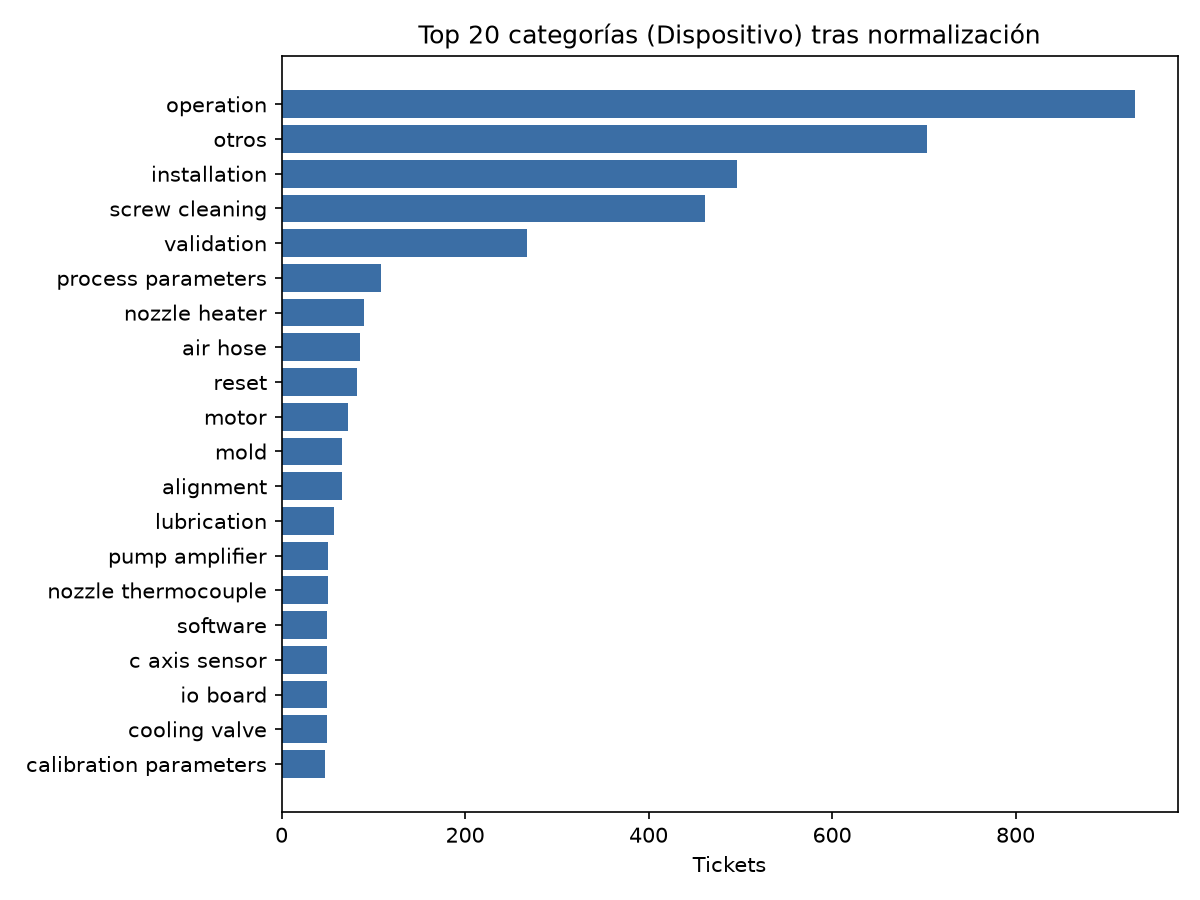
\includegraphics[width=\columnwidth]{fig_distribucion.png}}
\caption{Distribución y frecuencia de tickets por categoría de Dispositivo tras unificar mayúsculas y espacios (escala logarítmica). Se marca la línea punteada con el umbral de 10 ejemplos usado para agrupar clases minoritarias en Otros.}
\label{fig:dist_categorias}
\end{figure}

\begin{figure}[htbp]
\centerline{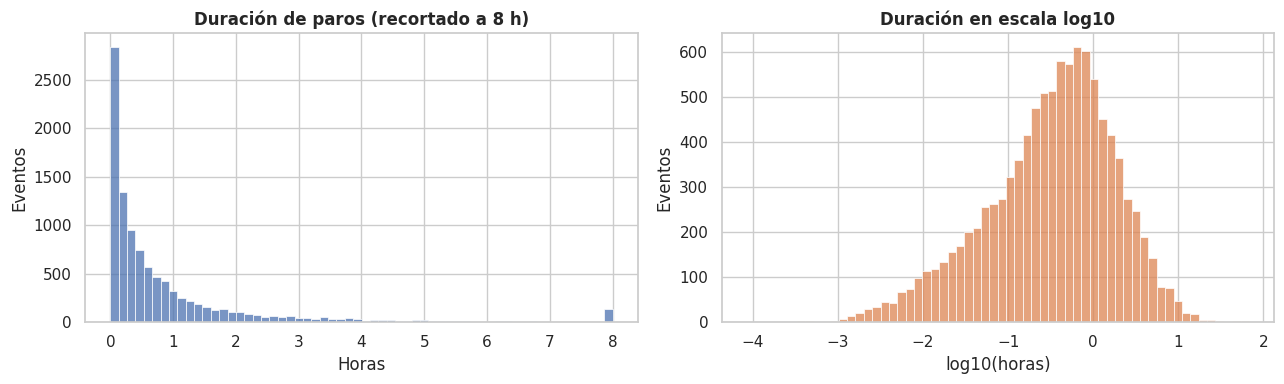
\includegraphics[width=\columnwidth]{fig_downtime_dist.png}}
\caption{Distribución de la duración de los paros: (a) en horas y (b) en escala logarítmica.}
\label{fig:dist_downtime}
\end{figure}

\begin{figure}[htbp]
\centerline{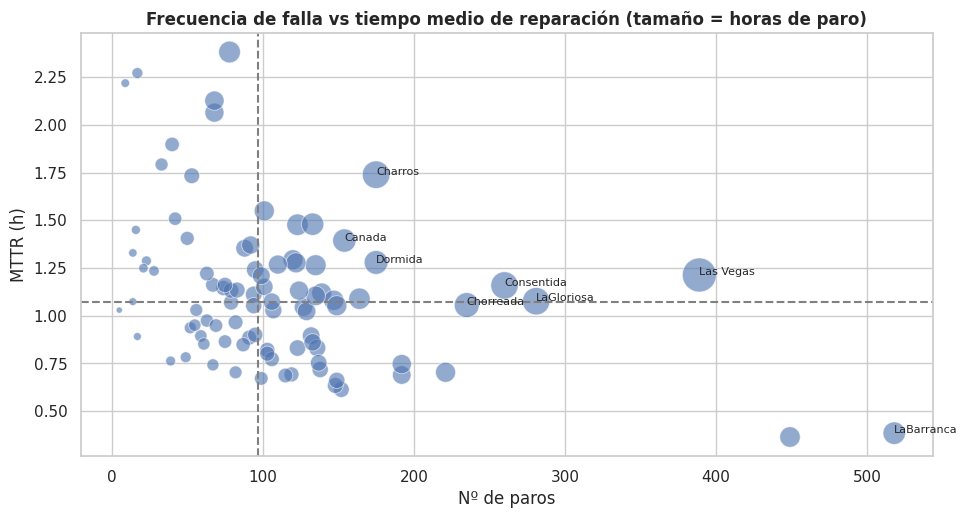
\includegraphics[width=\columnwidth]{fig_mttr_scatter.png}}
\caption{Número de paros contra tiempo medio de reparación (MTTR) por máquina. El tamaño del punto indica las horas totales de paro y las líneas punteadas marcan las medianas.}
\label{fig:mttr_scatter}
\end{figure}

\begin{figure}[htbp]
\centerline{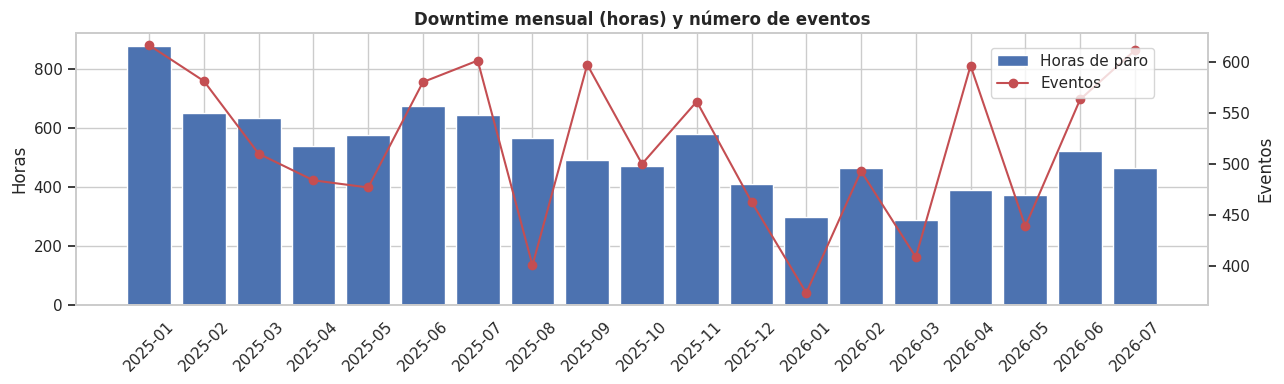
\includegraphics[width=\columnwidth]{fig_series_tiempo.png}}
\caption{Horas de paro (barras) y número de paros (línea) por mes, de enero de 2025 a julio de 2026. Se excluye agosto de 2026 por estar incompleto.}
\label{fig:series_tiempo}
\end{figure}

\section{Conclusiones Preliminares y Trabajo Futuro}
La introducción, la definición de los problemas, la descripción del dataset y el análisis exploratorio muestran que los datos sí permiten construir los modelos propuestos. La unión de 4,928 tickets entre ambas fuentes, los 5,222 tickets con texto y categoría, y la limpieza de los registros sin clasificar son la base para las siguientes etapas:
\begin{enumerate}
    \item \textbf{Agrupamiento de máquinas} ($k$-means~\cite{macqueen1967} y clustering jerárquico~\cite{ward1963}) con indicadores de confiabilidad ($MTBF$, $MTTR$, frecuencia de paros y \% de paros en cambios de modelo), para identificar los equipos que requieren atención, que es la prioridad del socio formador. El $MTBF$ se recalculará con las horas reales de operación de cada máquina.
    \item \textbf{Modelos de regresión y ensamble} (Random Forest~\cite{breiman2001}, LightGBM~\cite{ke2017} y XGBoost~\cite{chen2016}) para predecir el número de paros y las horas de paro por máquina, así como la duración esperada de un paro al momento del reporte.
    \item \textbf{Clasificación del texto de cierre} (columna Q) en la categoría Dispositivo (columna AB) con TF-IDF~\cite{salton1988} de palabras y de caracteres, regresión logística~\cite{cox1958} y Naive Bayes~\cite{mccallum1998}, implementados con scikit-learn~\cite{pedregosa2011}, y exploración de modelos de lenguaje~\cite{goodfellow2016}.
\end{enumerate}

\begin{thebibliography}{00}
\bibitem{mobley2002} R. K. Mobley, \textit{An Introduction to Predictive Maintenance}, 2nd ed. Butterworth-Heinemann, 2002.
\bibitem{jardine2006} A. K. S. Jardine, D. Lin, and D. Banjevic, ``A review on machinery diagnostics and prognostics implementing condition-based maintenance,'' \textit{Mechanical Systems and Signal Processing}, vol. 20, no. 7, pp. 1483--1510, 2006.
\bibitem{hastie2009} T. Hastie, R. Tibshirani, and J. Friedman, \textit{The Elements of Statistical Learning: Data Mining, Inference, and Prediction}, 2nd ed. Springer, 2009.
\bibitem{breiman2001} L. Breiman, ``Random forests,'' \textit{Machine Learning}, vol. 45, no. 1, pp. 5--32, 2001.
\bibitem{friedman2001} J. H. Friedman, ``Greedy function approximation: A gradient boosting machine,'' \textit{The Annals of Statistics}, vol. 29, no. 5, pp. 1189--1232, 2001.
\bibitem{macqueen1967} J. MacQueen, ``Some methods for classification and analysis of multivariate observations,'' in \textit{Proc. 5th Berkeley Symp. Mathematical Statistics and Probability}, vol. 1, 1967, pp. 281--297.
\bibitem{ward1963} J. H. Ward, ``Hierarchical grouping to optimize an objective function,'' \textit{Journal of the American Statistical Association}, vol. 58, no. 301, pp. 236--244, 1963.
\bibitem{ke2017} G. Ke \textit{et al.}, ``LightGBM: A highly efficient gradient boosting decision tree,'' in \textit{Advances in Neural Information Processing Systems}, vol. 30, 2017, pp. 3146--3154.
\bibitem{chen2016} T. Chen and C. Guestrin, ``XGBoost: A scalable tree boosting system,'' in \textit{Proc. 22nd ACM SIGKDD Int. Conf. Knowledge Discovery and Data Mining}, 2016, pp. 785--794.
\bibitem{salton1988} G. Salton and C. Buckley, ``Term-weighting approaches in automatic text retrieval,'' \textit{Information Processing \& Management}, vol. 24, no. 5, pp. 513--523, 1988.
\bibitem{cox1958} D. R. Cox, ``The regression analysis of binary sequences,'' \textit{Journal of the Royal Statistical Society: Series B}, vol. 20, no. 2, pp. 215--242, 1958.
\bibitem{mccallum1998} A. McCallum and K. Nigam, ``A comparison of event models for naive Bayes text classification,'' in \textit{AAAI-98 Workshop on Learning for Text Categorization}, 1998, pp. 41--48.
\bibitem{pedregosa2011} F. Pedregosa \textit{et al.}, ``Scikit-learn: Machine learning in Python,'' \textit{Journal of Machine Learning Research}, vol. 12, pp. 2825--2830, 2011.
\bibitem{goodfellow2016} I. Goodfellow, Y. Bengio, and A. Courville, \textit{Deep Learning}. MIT Press, 2016.
\end{thebibliography}

\end{document}

